\begin{frame}
    \frametitle{LiDAR 2D}
    
    
    \begin{figure}[!h]
        \centering
        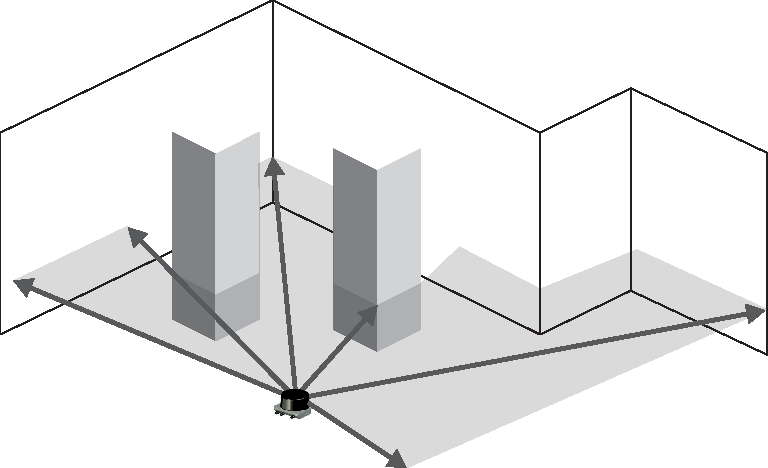
\includegraphics[width=\columnwidth]{images/lidar_example.pdf}
    \end{figure}

    \note{imagen extraida de:  https://cdn.sick.com/media/docs/3/43/443/operating_instructions_lms1104c_111031s01_2d_lidar_sensors_en_im0079443.pdf}

\end{frame}

\begin{frame}
    \frametitle{LiDAR 2D}
    
    \begin{figure}[!h]
        \centering
        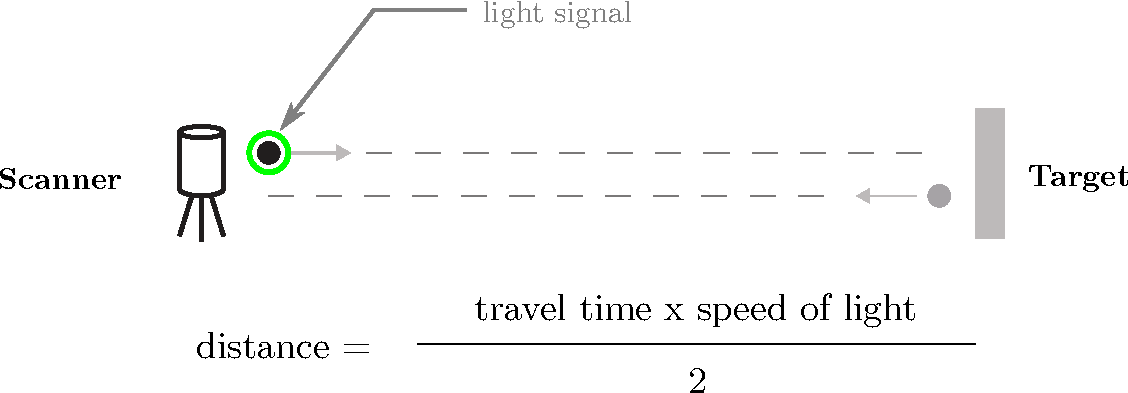
\includegraphics[width=0.8\columnwidth]{images/lidar_concept.pdf}
    \end{figure}
    \footnotesize
    \begin{block}{Principio de funcionamiento}
     Un LiDAR (\emph{Light Detection And Ranging}) o Laser Rangefinder emite pulsos de luz mediante un diodo láser (infrarrojo). Si el rayo láser es reflejado por un objeto, el rayo reflejado es recibido por el sensor.
     
     La distancia al objeto se calcula en base al tiempo que el haz de luz pulsada requiere para ser reflejada y recibida por el sensor.
    \end{block}
    
    \begin{itemize}
        \item Extereoceptivo
        \item Activo
        \item Mide distancia y ángulo a cada punto (coordenadas polares)
        \item Unidad de medición $\si{\degree\second}$ o Revoluciones por Minuto (RPM)
    \end{itemize}

    \note{Información extraida de:  https://cdn.sick.com/media/docs/3/43/443/operating_instructions_lms1104c_111031s01_2d_lidar_sensors_en_im0079443.pdf}

\end{frame}

\begin{frame}
    \frametitle{LiDAR 2D}
    
    \begin{figure}[!h]
        \centering
        \subfloat[]
        {
            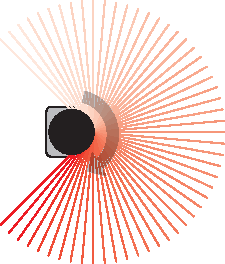
\includegraphics[width=0.4\columnwidth]{images/lidar_range.pdf}
        }
        \subfloat[]
        {
            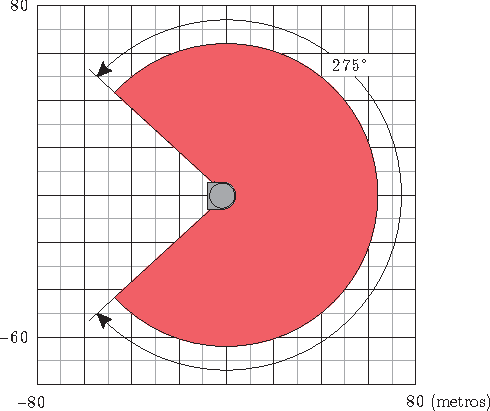
\includegraphics[width=0.55\columnwidth]{images/lidar_range2.pdf}
        }
    \end{figure}

    \note{imagenes extraida de:  https://cdn.sick.com/media/docs/3/43/443/operating_instructions_lms1104c_111031s01_2d_lidar_sensors_en_im0079443.pdf}
 
\end{frame}

\begin{frame}
    \frametitle{LiDAR 3D}

    \begin{figure}[!h]
        \centering
        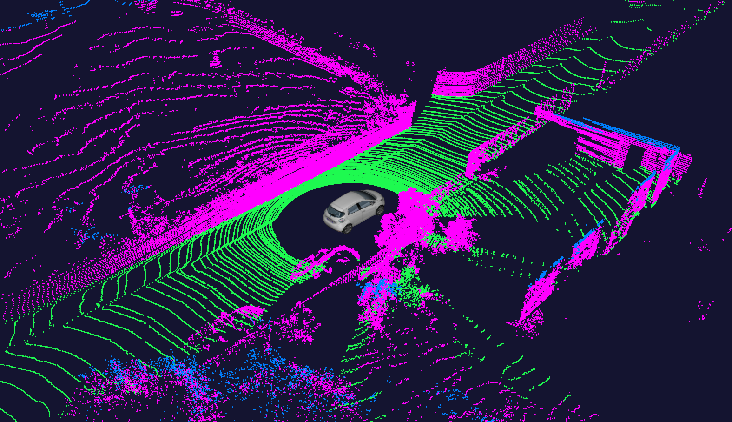
\includegraphics[width=\columnwidth]{images/lidar3d.png}
    \end{figure}

\end{frame}